\documentclass{beamer}
\usepackage{tfrupee} % Include tfrupee package
\usepackage{amsmath,amssymb,amsfonts,amsthm}
\usepackage{graphicx}
\usepackage{enumitem}
\usepackage{mathtools}
\usepackage{gensymb}

\title{Construction of triangle}
\author{AI24BTECH11006 - Bugada Roopansha}
\institute{IIT Hyderabad}
\date{November 6, 2024}

\begin{document}

\begin{frame}
    \titlepage
\end{frame}

\begin{frame}{Question}
    \textbf{Construct a right triangle when one side is 3.5 cm, and the sum of the other side and the hypotenuse is 5.5 cm.}
    
\end{frame}

\begin{frame}{Solution: Parameters}
    \begin{table}[h!]
        \centering
        \begin{tabular}{|c|c|c|}
            \hline
            \textbf{Segment} & \textbf{Norm} & \textbf{Angles} \\ \hline
            \( ||AB|| \) & 3.5 & $\theta_1$ \\ \hline
            \( ||BC|| \) & Distance between B and C & $\theta_2$ \\ \hline
            \( ||AC|| \) & Distance between C and A & $\theta_3$ \\ \hline
        \end{tabular}
        \caption{Input parameters}
    \end{table}
\end{frame}

\begin{frame}{Solution: Calculations}
    Given:
    \[
    ||AB|| = 3.5 \, \text{cm}, \quad ||BC|| + ||AC|| = 5.5 \, \text{cm}
    \]
    
    \[
    \implies ||AC|| = \sqrt{||AB||^2 + ||BC||^2}
    \]
    
    \[
    \implies 5.5 - ||BC|| = \sqrt{(3.5)^2 + ||BC||^2}
    \]
\end{frame}

\begin{frame}{Solution: Further Calculations}
    Expanding the equation:
    \[
    \implies (5.5 - ||BC||)^2 = (3.5)^2 + ||BC||^2
    \]
    
    Simplifying:
    \[
    \implies ||BC|| = \frac{18}{11} \approx 1.64 \, \text{cm}
    \]
    
    \[
    \implies ||AC|| = 5.5 - ||BC|| \approx 3.86 \, \text{cm}
    \]
\end{frame}

\begin{frame}{Solution: Final Calculations}
    Using vectors:
    \[
    \mathbf{u} = \begin{bmatrix} 3.5 \\ 0 \end{bmatrix}, \quad \mathbf{c} = \begin{bmatrix} 3.5 \\ 1.64 \end{bmatrix}
    \]
    
    \[
    \cos(\theta) = \frac{12.25}{3.5 \cdot \sqrt{3.5^2 + 1.64^2}}
    \]
    
    \[
    \theta \approx 34.89^\circ
    \]
\end{frame}

\begin{frame}{Diagram}
    \begin{figure}[h!]
        \centering
        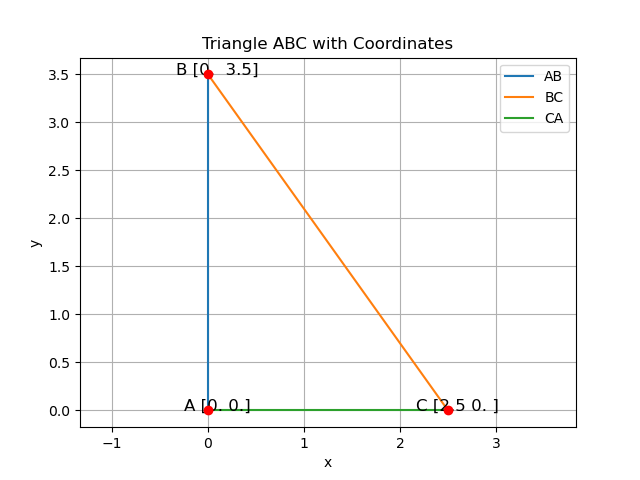
\includegraphics[width=0.9\textwidth]{fig.png} % Replace with your triangle diagram
        \caption{Right triangle with one side of 3.5 cm and the sum of the other side and hypotenuse equal to 5.5 cm.}
    \end{figure}
\end{frame}

\end{document}

